%!TEX root = thesis.tex

\chapter{Introduction}
\label{chap:intro}

\tikz \draw[-latex,ultra thick]  node[right,fill=yellow,append after command={(a.south west) -- ($(a.south west)!0.65!(a.south east)$)},label={[inner sep=0]south east:$100$},
label={[inner sep=0]south west:$0$}] (a) {Current status: 65\%: Delayed until the finish of Chap.3};
\vspace{1cm}



The success of the technological advances often can be associated with an unprecedented convenience that they bring in. At the heart of this convenience lies the ability to relax the limitations of the human body to a certain extent. From this point of view, it is not a surprise that the three most prominent technological wonders of the last century, namely the \emph{Television}, the \emph{Telephone} and the \emph{radio} (which was originally called ``radiotelegraphy"), bears the same Greek prefix \emph{tele-} which corresponds to ``\emph{at a distance}" in our context. This shows that there is something of extreme importance about our drive to extend our capabilities beyond the constraints that our bodies impose.


It is quite remarkable, in retrospect, that these ``gadgets" did not perish but rather kept on evolving since initially they were far from perfect. Quite the contrary, they were hardly operational. Even the commercialized version of the early TVs had a narrow bandwidth and minimum image quality. Similarly radio and telephone was barely transmitting sensible information as far as the signal-to-noise ratio is concerned. Nevertheless, they have provided the ways of communication which were unimaginable before their time. Therefore the added value dominated the shortcomings and even though they were quite imperfect, we kept using them. The important lesson to be learned was that a technology should not be judged by its imperfections but rather should be weighed by its contribution in this context or the convenience that is brought in by using it.  

The success is also related to the fact that these technologies mainly relied on the human brain itself at their early stages. For example, the human brain did most of the noise filtering and data recovery by just guessing the missing pieces and identifying patterns from the signal brought by the respective medium. Today, with our smart mobile phones and 3D LED TVs, we can assume that the computational load on the human brain is drastically reduced. In other words, it's true that we are still identifying patterns and utilizing the relevant parts of our brain to make sense of a TV broadcast\footnote{Pun intended.}. However, we don't need to use a higher level of concentration to reconstruct the words that we hear or to identify the image on the display thanks to the high quality output. We can not exaggerate the importance of the human brain and its immersion power. 

It seems that we are on the same track with the technological developments involving our touch sense. Considering the importance of our touch sense in any given situation, the added value of extending of our perception in this modality needs no motivation. Take the most familiar example: the vibrating mobile phone in the silent mode in our pocket. This is a very important example since every individual learns what that vibration might mean, either an SMS or a call, depending on the vibrational pattern. This means that the touch sense can be used to convey messages and more importantly we can process those messages for inference. 


This type of information said to be received via the haptic channel (or the collaborative use of tactile and proprioceptive modalities). Note that, we use the term ``touch sense'' pretty vaguely as a shortcut and we leave it to the experts of the field to define the sophisticated mechanisms (pertaining to the somatosensory system) that we utilize when we manipulate objects, say with our bare hands. 


Since our skin and muscles form one of most sophisticated and complex sensory systems, the somatosensory system, the brain can easily interpret the slightest changes and this extra signal processing power gives us a chance to hack into this system by providing artificial inputs. Still, it is rather conspicuous that this is impossible to achieve with today's technology. The essential complication is twofold; the high sensitivity of the very same sensory system makes it difficult to fake or mimic a natural phenomenon by artificial means and on the other hand we don't have a well-defined mapping from the to-be-created sensation to the required excitation signals. Moreover, even if we have such mappings available, the related hardware must execute the computed haptic signal profiles perfectly which is generally not the case.

Then, we could simply ask \emph{Why bother?} 


\section{The Objectives}

We first give an opiniated view about the objectives of the technology (as we foresee from a narrow ``today's'' perspective) and later on, define our microscopic focus of this thesis in this vast generality. This would hopefully give some perspective to what follows in the later sections.  


The touch related applications are diverse. The diversity is not only in terms of sensation they are related to (texture, shape etc.) but also how they encode the information and transmit via various modalities (e.g. vibrational patterns in mobile electronics, variable resistance to motion in game consoles and steering wheels etc.). There is no particular reason to limit ourselves with the daily needs or even luxurious demands regarding our touch sense as mobile phones taught us that a vibration in our pocket means a contact request from someone which is hardly ever related to the touch sense. This should be pretty awkward to experience if someone actually would come and shake our pockets to draw our attention (unless it is socially accepted). Therefore, we have devised a way to translate one particular message into another by simply teaching ourselves and getting used to it. Note that, we still don't have any idea about the distant person on the line however, once the call is accepted we suddenly require a higher level of detail. Hence, it does not seem improbable that other types of physical units in terms temperature, light intensity etc. being converted into pressure or tactile patterns in time domain.

Hence, it is our belief that the crux of this technology is establishing a interpretable protocol between our brain and the machine but not exactly reflecting the particular state of some distant or virtual physical medium. 
This would be the main argument of this thesis when we distinguish our approach with its comparable counterparts. For this reason, we would like to narrow down our focus further by defining different types of touch related concepts.






\newcolumntype{C}{>{\centering\arraybackslash}p{1.9cm}}%
\begin{table}%
\centering
\caption[Functional Features of Cutanous Mechanoreceptors]{Functional Features of Cutanous Mechanoreceptors (Adapted from \cite{idareview})}
{\tiny
\pgfplotstabletypeset[
column type=C,
every head row/.style={before row={\toprule},after row=\midrule,},
every last row/.style={after row=\bottomrule},
%columns/person/.style ={column name=},
%columns/singGaeilge/.style ={column name=Gaeilge},
%columns/pluralGaeilge/.style={column name=Gaeilge},
%columns/singEnglish/.style ={column name=English},
%columns/pluralEnglish/.style={column name=English},
every even row/.style={before row={\rowcolor[gray]{0.9}}},
col sep=&,row sep=\\,
string type,
]{
Feature	                   &Meissner Corpuscles (FAI) &Pacinian Corpuscles (FAII) &Merkel's Disks (SAI) &Ruffini Endings (SAII)\\
Rate of adaptation         &Rapid &Rapid &Slow	&Slow\\
Location                   &Superficial dermis &Dermis and subcutaneous &Basal epidermis &Dermis and subcutaneous\\
Mean receptive area        &\SI{13}{\milli\metre\squared} &\SI{101}{\milli\metre\squared} &\SI{11}{\milli\metre\squared} &\SI{59}{\milli\metre\squared}\\
Spatial resolution         &Poor&Very poor&Good&Fair\\
Sensory units              &43\%&13\%&25\%&19\%\\
Response frequency range   &\SIrange{10}{200}{\hertz}&\SIrange{70}{1000}{\hertz} &\SIrange{0.4}{100}{\hertz} &\SIrange{0.4}{100}{\hertz} \\
Min. threshold frequency   &\SI{40}{\hertz}&\SIrange{200}{250}{\hertz} &\SI{50}{\hertz}&\SI{50}{\hertz}\\
Sensitive to temperature   &No&Yes&Yes&At $>\SI{100}{\hertz}$\\
Spatial summation          &Yes&No&No&Unknown\\
Temporal summation         &Yes&No&No&Yes\\
Physical parameter sensed  &Skin curvature, velocity, local shape,flutter, slip &Vibration, slip, acceleration &Skin curvature, local shape, pressure&Skin stretch, local force\\
}
}% Closes the \tiny group
\label{tab:mechano}
\end{table}
\subsection{A Terminological Classification}

As we mentioned above, the somatosensory system is quite complex and there are different layers of sensory mechanisms that contribute to the overall perception. The main two branches of technology relating to the touch perception is the tactile and kinesthetic  feedback. The terminology is yet to reach a steady-state standard however what follows below is plausible considering the variations and nuances found in the literature. Since there is no fixed definition for such perception we would use a rough  classification based on the amplitude-frequency of the motion. We have to emphasize that this classification is completely conceptual and only serves to exclude the parts that is not studied in this thesis. Therefore, we refer the reader to the authoritative resources of the involved physiology. 

Typically, the touch perception is classified into two groups. Tactile feedback and kinesthetic (proprioceptive) feedback. For practical purposes, one can use the analogy of parallel connected a high-pass and a low-pass filters. As shown in \Cref{tab:mechano}, and also surveyed in \cite{kontarinis}, there are four main types of mechanisms that are utilized for the force and texture sensing with varying operating conditions and spatial authority. Although all contribute to the high frequency stimulus perception with varying levels, slowly adapting receptors are mainly tuned to detect the low frequency information range (up to \SI{30}{\hertz}). The fast adapting Meissner(FAI) and Pacinian(FAII) Corpuscles can be excited in the frequency range of \SIrange{10}{60}{\hertz} and $\SIrange{60}{1000}{\hertz}$ respectively. Thus, small-area receptors (Meissner) are excited with rate of skin deformation whereas relatively large-area receptors (Pacinian) are with acceleration of the skin. Moreover, FAI units are located closer to the skin surface, have high unit density with small surface area forming a grid of sensors. On the other hand, FAII units are located in the subcutaneous tissue and work as a single load cell with relatively large surface area. This allows experts to assume that FAI units are mainly responsible for spatial information about the skin deformation and FAII units are responsible for the high frequency information. It is also noted that each of these are reported to have response delays \SIrange{50}{500}{\milli\second} \cite{idareview}. Another interesting note in \cite{kontarinis} is that due to their single unit nature FAII units offers the possibility to provide high frequency information with a single vibration display but for FIA units it is more appropriate to supply an array of haptic displays for lower frequency range.  







\subsubsection{Tactile Feedback}
The most striking example is probably the Braille system used by visually impaired or disabled individuals as shown in \Cref{fig:braille}. The average reading speed with Braille system is about 125-150 words per minute (\cite{americanblind}) in contrast with 200-250 words per minute by eyesight. 

\begin{figure}%
\centering
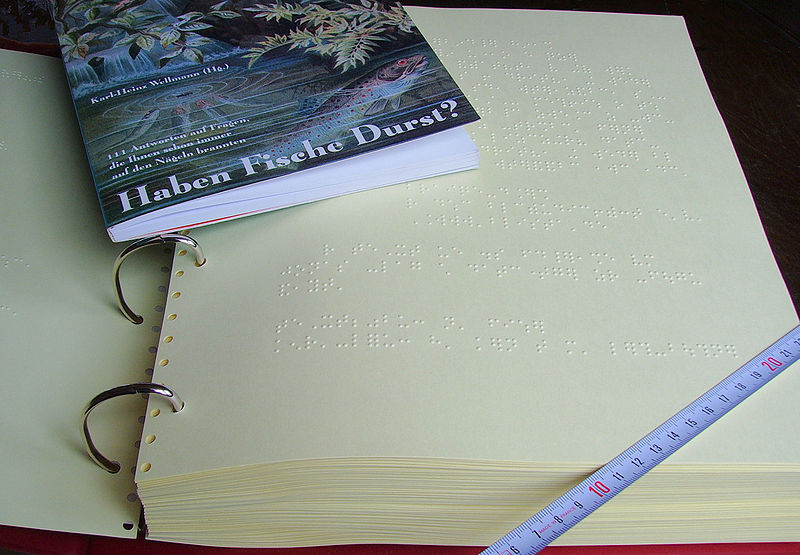
\includegraphics[width=0.8\columnwidth]{\impath/intro/braille.jpg}%
\caption[The length comparison of the same content in the form of Braille and 
regular text]{The length comparison of the same content in the form of Braille and 
regular text (Source: Karl-Heinz Wellmann, 
\href{http://de.wikipedia.org/wiki/Brailleschrift}{[Wikipedia:Brailleschrift]})}%
\label{fig:braille}%
\end{figure}

Most of today's technological devices utilize this channel to send and receive information. Many mobile phone applications and a few gaming consoles such as Nintendo Wii\raisebox{0.5ex}{\scriptsize\texttrademark}, Sony Playstation\raisebox{0.5ex}{\scriptsize\texttrademark} etc., utilize short vibrational patterns to alert the user that some action has been performed e.g. the user hovers over a hot spot on the screen or some moving object hits an obstacle etc. 


\subsubsection{Teleoperation}

\pagebreak[1]

\subsubsection{Bilateral Teleoperation}

\pagebreak[1]
\subsubsection{Haptics}
\pagebreak[1]
\subsubsection{Virtual Reality}
\pagebreak[1]



\subsection{Objective of This Thesis}
\pagebreak[1]


%Transparency TV den istense renkler super olsun falan komple sacma. 